\documentclass[12pt]{article}

\title{Activity 10: Classes and UML}
\author{Chris Mayfield and Helen Hu}
\date{Spring 2018}

%\ProvidesPackage{cspogil}

% fonts
\usepackage[utf8]{inputenc}
\usepackage[T1]{fontenc}
\usepackage{mathpazo}

% spacing
\usepackage[margin=2cm]{geometry}
\renewcommand{\arraystretch}{1.4}
\setlength{\parindent}{0pt}

% orphans and widows
\clubpenalty=10000
\widowpenalty=10000
\pagestyle{empty}

% figures and tables
\usepackage{graphicx}
\usepackage{multicol}
\usepackage{tabularx}
\usepackage{wrapfig}

% fixed-width columns
\usepackage{array}
\newcolumntype{L}[1]{>{\raggedright\let\newline\\\arraybackslash\hspace{0pt}}m{#1}}
\newcolumntype{C}[1]{>{\centering\let\newline\\\arraybackslash\hspace{0pt}}m{#1}}
\newcolumntype{R}[1]{>{\raggedleft\let\newline\\\arraybackslash\hspace{0pt}}m{#1}}

% include paths
\makeatletter
\def\input@path{{Models/}{../../Models/}}
\graphicspath{{Models/}{../../Models/}}
\makeatother

% colors
\usepackage[svgnames,table]{xcolor}
\definecolor{bgcolor}{HTML}{FAFAFA}
\definecolor{comment}{HTML}{007C00}
\definecolor{keyword}{HTML}{0000FF}
\definecolor{strings}{HTML}{B20000}

% table headers
\newcommand{\tr}{\bf\cellcolor{Yellow!10}}

% syntax highlighting
\usepackage{textcomp}
\usepackage{listings}
\lstset{
    basicstyle=\ttfamily\color{black},
    backgroundcolor=\color{bgcolor},
    numberstyle=\scriptsize\color{comment},
    commentstyle=\color{comment},
    keywordstyle=\color{keyword},
    stringstyle=\color{strings},
    columns=fullflexible,
    keepspaces=true,
    showlines=true,
    showstringspaces=false,
    upquote=true
}

% code environments
\newcommand{\java}[1]{\lstinline[language=java]{#1}}%[
\lstnewenvironment{javalst}{\lstset{language=java,backgroundcolor=}}{}
\lstnewenvironment{javabox}{\lstset{language=java,frame=single,numbers=left}\quote}{\endquote}

% PDF properties
\usepackage[pdftex]{hyperref}
\urlstyle{same}
\makeatletter
\hypersetup{
  pdftitle={\@title},
  pdfauthor={\@author},
  pdfsubject={\@date},
  pdfkeywords={},
  bookmarksopen=false,
  colorlinks=true,
  citecolor=black,
  filecolor=black,
  linkcolor=black,
  urlcolor=blue
}
\makeatother

% titles
\makeatletter
\renewcommand{\maketitle}{\begin{center}\LARGE\@title\end{center}}
\makeatother

% boxes [optional height]
\newcommand{\emptybox}[1][10em]{
\vspace{1em}
\begin{tabularx}{\linewidth}{|X|}
\hline\\[#1]\hline
\end{tabularx}}

% models
\newcommand{\model}[1]{\section{#1}\nopagebreak}
\renewcommand{\thesection}{Model~\arabic{section}}

% questions
\newcommand{\quest}[1]{\subsection*{Questions~ (#1)}}
\newcounter{question}
\newcommand{\Q}{\vspace{1em}\refstepcounter{question}\arabic{question}.~ }
\renewcommand{\thequestion}{\#\arabic{question}}

% sub-question lists
\usepackage{enumitem}
\setenumerate[1]{label=\alph*)}
\setlist{itemsep=1em,after=\vspace{1ex}}

% inline answers
\definecolor{answers}{HTML}{C0C0C0}
\newcommand{\ans}[1]{%
\ifdefined\Student
    \leavevmode\phantom{~~\textcolor{answers}{#1}}
\else
    ~~\textcolor{answers}{#1}
\fi}

% longer answers [optional height]
\newsavebox{\ansbox}
\newenvironment{answer}[1][4em]{
\nopagebreak
\begin{lrbox}{\ansbox}
\begin{minipage}[t][#1]{\linewidth}
\color{answers}
}{
\end{minipage}
\end{lrbox}
\ifdefined\Student
    \phantom{\usebox{\ansbox}}%
\else
    \usebox{\ansbox}%
\fi}


\begin{document}

\maketitle

The \java{String} class provides methods for working with text.
The \java{Random} class provides methods for generating random numbers.
In this activity, you'll learn how to make your own classes that represent everyday objects.

\guide{
  \item Define the terms: attribute, method, constructor, instance.
  \item Implement non-static methods based on a UML diagram.
  \item Distinguish between static, instance, parameter, and local variables.
}{
  \item Writing method signatures exactly as shown in a UML diagram. (Information Processing)
}{
\ref{die-class.tex} is primarily about introducing object-oriented vocabulary.
As you walk around, keep an eye on \ref{dievar}.
Some students may incorrectly write \texttt{int lucky}, and if that happens, have them re-read the text in \ref{die-class.tex}.
For reporting out, have presenters of neighboring teams compare their answers and ask questions as needed.

\ref{circle-class.tex} asks students to implement a \texttt{Circle} class, one method at a time.
After they complete \ref{circmain}, show Circle.java on the projector and step through the code beginning from \texttt{main}.
It may be helpful to use \href{http://pythontutor.com/java.html}{Java Tutor} to illustrate how \texttt{Circle} objects are created on the heap.

\ref{variable-scope.tex} presents a slightly different circle class named \texttt{SwapCircle}.
Have students work through the first questions as quickly as possible so they can spend time on \ref{predict}.
You'll need about ten minutes at the end of class to walk students through the solution, again using Java Tutor or similar tool.
}

\model{The Die Class}

When you define a \java{class} in Java, you are defining a new type.
Classes have \emph{attributes} (data) and \emph{methods} (code).
A \emph{class diagram} is a graphical summary of the attributes and methods.

\vspace{1em}
\begin{quote}
\hfill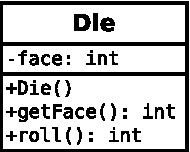
\includegraphics{Die.pdf}
\vspace*{-84pt}

\begin{javalst}
/**
 * Simulates a Die object.
 */
public class Die {
    
    private int face;
    
    /**
     * Constructs a new die with a random face value.
     */
    public Die() {
        this.face = 1;
    }
    
    /**
     * Gets the current face value of the die.
     *
     * @return current face value of the die
     */
    public int getFace() {
        return this.face;
    }
    
    /**
     * Simulates the roll of the die.
     *
     * @return new face value of the die
     */
    public int roll() {
        this.face = (int) (Math.random() * 6) + 1;
        return this.face;
    }
    
}
\end{javalst}

\vspace*{-128pt}
% https://commons.wikimedia.org/wiki/File:2-Dice-Icon.svg
\hfill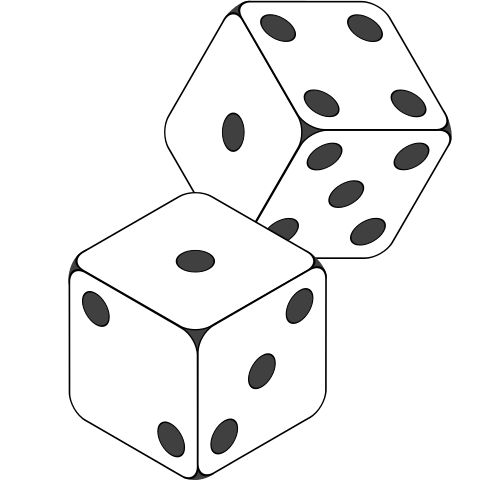
\includegraphics[width=2in]{dice.png}
\end{quote}


\quest{10 min}


\Q What are the attributes of \java{Die}? What are the methods?

\begin{answer}
The only attribute is \java{face}. The methods are \java{Die}, \java{roll}, and \java{getFace}.
\end{answer}


\Q In the class diagram, what do the \java{-} and \java{+} symbols represent? What does the \java{:} represent?

\begin{answer}
Plus means {\tt public}, minus means {\tt private}, and colon refers to the data type.
\end{answer}


\Q \label{dievar}
Write a statement that \emph{declares} a \java{Die} variable named \java{lucky}.

\begin{answer}
\tt Die lucky;
\end{answer}


\Q Each \emph{instance} of a class (in memory) is called an object. Write a statement that \emph{instantiates} a \java{new} \java{Die} object and assigns it to \java{lucky}.

\begin{answer}
\tt lucky = new Die();
\end{answer}


\Q When you instantiate an object, you invoke a \emph{constructor}.
This method has no return type and has the same name as the class itself. What does the \java{Die} constructor do?

\begin{answer}
It initializes the \java{face} attribute to 1.
(Without this constructor, the default value would be 0, which is invalid for dice.)
\end{answer}


\Q Notice how the \java{roll} method refers to \java{face}, yet that variable is not declared in the method. What does the \java{roll} method change, in terms of the \java{Die} object?

\begin{answer}
It updates the value of the \java{face} attribute.
\end{answer}


\Q What is the purpose of the \java{getFace} method? Show how you would use it in a \java{main} method of another class.

\begin{answer}
In a {\tt main} method, you would do something like: {\tt System.out.println(lucky.getFace());}
\end{answer}

\model{The Circle Class}

Unified Modeling Language (UML) provides a way of graphically illustrating a class’s design, independent of the programming language.

\begin{center}
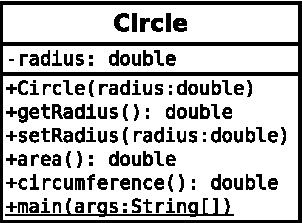
\includegraphics{Circle.pdf}
\end{center}


\quest{15 min}


\Q What are the attributes and methods of \java{Circle}, and what is their \emph{visibility}?

\begin{answer}
The attribute \java{radius} is private, and the methods \java{Circle}, \java{area}, \java{circumference}, \java{getRadius}, and \java{setRadius} are public.
\end{answer}


\Q Based on \ref{die-class.tex} and \ref{\currfilename}, what is typically \java{public} and what is typically \java{private}?

\begin{answer}
Attributes are typically private, and methods are typically public.
\end{answer}


\Q How would you declare a variable named \java{unit} that is a \java{Circle} object?
How would you instantiate a circle with a radius of 1.0 and assign it to \java{unit}?

\begin{answer}
\tt Circle unit;

\tt unit = new Circle(1.0);
\end{answer}


\Q Write the code (inside {\tt Circle.java}) that declares the \java{radius} attribute.

\begin{answer}
\tt private double radius;
\end{answer}


\Q Write the code for \java{getRadius}. (Don't worry about Javadoc comments for this activity.)

\begin{answer}[6em]
\begin{javaans}
    public double getRadius() {
        return this.radius;
    }
\end{javaans}
\end{answer}


\Q Write the code for \java{setRadius}. Note there are two variables named \java{radius}: the parameter of \java{setRadius}, and \java{this.radius} for the object itself. Before you set the radius, first check if the parameter is negative, and if it is, set \java{this.radius} to zero instead.

\begin{answer}[12em]
\begin{javaans}
    public void setRadius(double radius) {
        if (radius >= 0) {
            this.radius = radius;
        }
        else {
            this.radius = 0;
        }
    }
\end{javaans}
\end{answer}


\Q Write the complete code for \java{area} and \java{circumference}.
The area of a circle is $\pi r^2$, and the circumference is $2 \pi r$.
Ideally, each method should be one line of code.

\begin{answer}[12em]
\begin{javaans}
    public double area() {
        return Math.PI * radius * radius;
    }

    public double circumference() {
        return 2.0 * Math.PI * radius;
    }
\end{javaans}
\end{answer}


\Q \label{circmain}
Write a \java{main} method that creates a \java{Circle} object with a radius of 2.0 and displays its area and circumference on the screen.

\begin{answer}[8em]
\begin{javaans}
    public static void main(String[] args) {
        Circle big = new Circle(2.0);
        System.out.println("big area = " + big.area());
        System.out.println("big circ = " + big.circumference());
    }
\end{javaans}
\end{answer}

\newpage
\model{Variable Scope}
% based on Model 1 of "Improved Scope" activity by Helen Hu

As a team, first review and discuss the \java{SwapCircle} and \java{SwapDriver} classes found at the end of the questions.
Then identify the \emph{scope} of each variable based on the table below.

\begin{center}
\small
\begin{tabular}{|L{95pt}|L{125pt}|L{115pt}|L{105pt}|}
\hline
\tr &
\tr \textbf{Where declared?} &
\tr \textbf{Where used?} &
\tr \textbf{Example} \\
\hline
\textbf{static variables} \par (``class variables'') &
declared outside of all methods (typically at the start of the class) &
anywhere in the class (or in other classes if also \java{public}) &
\java{circleCount} in the \java{SwapCircle} class \\
\hline
\textbf{instance variables} \par (``attributes'') &
declared outside of all methods (typically after any static variables) &
any non-static method (or in static methods when another object has been created) &
\java{radius} in the \java{SwapCircle} class \\
\hline
\textbf{parameters} &
declared inside the ()'s of a method signature &
anywhere within the method where they are declared &
\java{radius} in the \java{SwapCircle} constructor \\
\hline
\textbf{local variables} &
declared inside a method (or inside another block of code, like a \java{for} loop) &
anywhere within the method or code block after they are declared &
\java{temp} in the \java{swapInts} method \\
\hline
\end{tabular}
\end{center}


\quest{20 min}


\Q Identify one static variable from the \java{SwapCircle} class.
\begin{enumerate}
\item What is the name and purpose of the variable?
\\ \ans{\java{circleCount} -- tracks the number of \java{SwapCircle} objects that have been created} \\[-2em]

\item What is the scope of the variable?
\\ \ans{{\tt private static} -- it can be used anywhere within the \java{SwapCircle} class only} \\[-2em]

\item What is one example of somewhere it cannot be used?
\\ \ans{\tt SwapDriver.main} \\[-2em]

\end{enumerate}


\Q Identify one instance variable from the \java{SwapCircle} class.
\begin{enumerate}
\item What is the name and purpose of the variable?
\\ \ans{\java{radius} -- stores the radius of {\tt this} SwapCircle} \\[-2em]

\item What is the scope of the variable?
\\ \ans{{\tt private} and non-{\tt static} -- it can only be used in \java{SwapCircle} in non-static contexts} \\[-2em]

\item What is one example of somewhere it cannot be used?
\\ \ans{\tt SwapDriver.main} \\[-2em]
\end{enumerate}


\newpage

\Q Identify an example of where an instance variable is used within a static method.
\begin{enumerate}
\item In which method does this occur?
\\ \ans{\java{radius} is used in the \java{swapCircles} method} \\[-2em]

\item Why is the method able to access these instance variables, even though they are private?
\\ \ans{\java{swapCircles} belongs to the \java{SwapCircle} class} \\[-2em]

\item Explain how this method is not a violation of the rule that instance variables cannot be accessed inside a static method.
\\ \ans{You can't use {\tt this}.radius in a {\tt static} method, but it's okay to use \java{c1.radius}} \\[-2em]
\end{enumerate}


\Q Identify one parameter from the \java{SwapCircle} class.
\begin{enumerate}
\item What is the name and purpose of the variable?
\\ \ans{Possible answers include: \java{radius} (in the constructor), \java{x} and \java{y}, \java{c1} and \java{c2}} \\[-2em]

\item What is the scope of the variable?
\\ \ans{The variable exists throughout the entire method (but not other methods).} \\[-2em]

\item Where can the variable not be used?
\\ \ans{It can't be used in other methods, e.g., you can't refer to \java{x} in \java{swapCircles}.} \\[-2em]
\end{enumerate}


\Q Identify one local variable from the \java{SwapCircle} class.
\begin{enumerate}
\item What is the name and purpose of the variable?
\\ \ans{Possible answers include: \java{temp} and \java{r} (both used for swapping values)} \\[-2em]

\item What is the scope of the variable?
\\ \ans{The variable exists from when it's declared until the end of the method.} \\[-2em]

\item Where can the variable not be used?
\\ \ans{It cannot be used in other methods and/or before it has been declared.} \\[-2em]
\end{enumerate}


\Q \label{predict}
In the space below, predict the output of the \java{SwapDriver} program.
Why are the results different when swapping integers and swapping objects?

\begin{answer}[14em]
\begin{minipage}{190pt}

\begin{javaans}
BEFORE swap:
a = 7
b = 4
    Inside swapInts
    swapping integers 7 and 4
    finished swapping 4 and 7
AFTER swap:
a = 7
b = 4
\end{javaans}

\end{minipage}
\hspace{1em}
\begin{minipage}{290pt}

\begin{javaans}
BEFORE swap:
first = Circle(7)
second = Circle(4)
	Inside swapCircles
	swapping circles Circle(7) and Circle(4)
	finished swapping Circle(4) and Circle(7)
AFTER swap:
first = Circle(4)
second = Circle(7)
\end{javaans}

\end{minipage}
\begin{javaans}
This program created 2 circles
\end{javaans}
\end{answer}


\newpage

\begin{center}
\large\bf SwapCircle.java
\vspace{-4pt}
\end{center}

\jafile{SwapCircle.java}


\newpage

\begin{center}
\large\bf SwapDriver.java
\vspace{-4pt}
\end{center}

\jafile{SwapDriver.java}


\end{document}
